\documentclass[14pt]{extarticle}

\usepackage{geometry}

\geometry{
    a4paper,
    top=2cm,
    bottom=2cm,
    left=2.5cm,
    right=1cm,
    nomarginpar,
    % showframe
}

\usepackage[utf8]{inputenc}
\usepackage[T2A]{fontenc}
\usepackage[english,russian]{babel}
\usepackage{indentfirst}

\usepackage{enumitem}
\usepackage{amssymb,amsmath}
\usepackage{graphicx}
\usepackage[caption=false]{subfig}
\usepackage{tikz}
\usetikzlibrary{patterns,intersections}
\usepackage{theoremref}

\graphicspath{{media/}}

\usepackage{amsthm}
\theoremstyle{plain}% Theorem-like structures provided by amsthm.sty
\newtheorem{theorem}{Theorem}[section]
\newtheorem{lemma}[theorem]{Lemma}
\newtheorem{corollary}[theorem]{Corollary}
\newtheorem{proposition}[theorem]{Proposition}

\theoremstyle{definition}
\newtheorem{definition}[theorem]{Definition}
\newtheorem{example}[theorem]{Example}

\theoremstyle{remark}
\newtheorem{remark}{Remark}
\newtheorem{notation}{Notation}
\newtheorem{condition}{Condition}

\usepackage{csquotes}

\usepackage[%
  parentracker=true,
  style=gost-numeric,
  defernumbers=true,
  % sorting=none,
]{biblatex}

\toggletrue{bbx:gostbibliography}

\addbibresource{ccp.bib}

\begin{document}

\thispagestyle{empty}
\begin{center}
{\small
Министерство науки и высшего образования Российской Федерации

Федеральное государственное автономное образовательное учреждение \\
высшего образования

\textbf{<<Уральский федеральный университет\\
имени первого Президента России Б.Н. Ельцина>>}
}

\vspace{0pt plus2fill}
\begin{flushright}
\begin{minipage}{0.5\linewidth}
  \centering
  \textit{На правах рукописи}

  \small {(подпись)}
\end{minipage}
\end{flushright}


\vspace{0pt plus4fill}
Уколов Станислав Сергеевич

\vspace{0pt plus1fill}
\textbf{
Эвристический алгоритм решения задачи непрерывной резки
}

\vspace{0pt plus1fill}
НАУЧНЫЙ ДОКЛАД

по результатам научно-квалификационной работы (диссертации)

\vspace{0pt plus2fill}
\begin{tabular}{l p{10cm}}
  Направление подготовки: &
  09.06.01
  "---
  <<Информатика и вычислительная техника>>
  \\
  Направленность: &
  05.13.12
  "---
  <<Системы автоматизации проектирования (в промышленности)>>
\end{tabular}

\vspace{0pt plus4fill}
\begin{flushright}
Научный руководитель:
профессор,
д.т.н.
\\
Петунин Александр Александрович
\end{flushright}

\vspace{0pt plus6fill}
Екатеринбург
\\
2020
\end{center}
\newpage

\tableofcontents
\newpage

\section{Введение}

См.
\cite{berlin2019}
и
\cite{bi07},
а также
\cite{Miskolc,Sozopol,Obuhovo}.

\section{Задача непрерывной резки -- Continuous Cutting Problem}

Рассмотрим Эквлидову плоскость
$\mathbb R ^ 2$
и на ней фигуру
$B$
(в большинстве практических случаев -- прямоугольник),
ограниченную замкнутым контуром.
Это -- модель листового материала,
подлежащего резке.
Пусть
$N$
попаркно непересекающихся плоских контуров
$\{C_1, C_2, ... C_N\}$
расположены внутри
$B$,
ограничивая
$n$
деталей
$\{A_1, A_2 ... A_n\}$.
Деталь может быть ограничена
одним или несколькими контурами
(одним внешним и несколькими отверстиями),
так что в общем случае
$n \leqslant N$.

Контуры
$C_i$
могут быть произвольной формы,
но мы будем рассматривать только
состоящие из
(конечного числа)
отрезков прямых линий и дуг окружностей,
так как именно такие геометрические примитивы
поддерживаются программным обеспечением
современных машин термической резки с ЧПУ.
Частный случай,
когда контура состоят только
из отрезков прямых,
сводится к одному из вариантов
задачи обхода прямоугольников
(Touring Polygon Problem, TPP),
см.
\cite{bi13}.

Далее,
внутри
$B$
(как правило, на границе)
выберем две точки и обозначим их
$M_0$, $M_{N + 1}$
(почти всегда $M_0 = M_{N + 1}$),
которые будут использоваться
как начало и конец
маршрута резки.

Задача непрерывной резки
(Continuous Cutting Problem, CCP)
состоит в поиске:
\begin{enumerate}
\item
$N$ штук точек врезки $M_i \in C_i, i \in \overline{1, N}$
\item
Последовательности обхода контуров
$C_i$,
то есть перестановки
$N$
элементов
$I = (i_1, i_2, ... i_N)$
\end{enumerate}

Результатом решения задачи будет являться маршрут
\begin{equation}
  \{M_0, M_{i_1}, M_{i_2}, \dots M_{i_N}, M_{N + 1}\}
\end{equation}
Целевая функция в данном случае сильно упрощается
по сравнению с общей задачей маршрутизации резки
и сводится фактически к минимизации длины холостого хода:

\begin{equation}
  \mathcal{L} = \sum_{j=0}^N|M_{i_j}M_{i_{j+1}}|
  \label{air-move-length}
\end{equation}
$$
\mathcal{L} \to \min
$$
где, для простоты записи мы полагаем
$M_{i_0} = M_0$,
$M_{i_{N + 1}} = M_{N + 1}$.

Кроме того,
мы наложим на решение дополнительное ограничение,
известное как
<<ограничение предшествования>>
(``precedence constraint'').
Хотя контуры
$C_i$
по условию не пересекаются,
они могут быть вложены друг в друга:
\( \tilde C_a \subset \tilde C_b \),
где
$\tilde C_a$
обозначает 2-мерную фигуру,
ограниченную контуром
$C_a$
(в более традиционных обозначениях
$C_a = \partial \tilde C_a$).
В общей задаче маршрутизации
режущего инструмента это
соответствует двум разным случаям
(наличие отверстий в деталях с одной стороны
и размещение меньших деталей в отверстиях больших),
но в нашем случае оба этих
варианта обрабатываются одинаково.

Если один контур расположен внутри другого,
то внутренний должен быть вырезан
(посещён)
ранее, чем внешний:
\( \tilde C_a \subset \tilde C_b \Rightarrow i_a < i_b \),
в перестановке
$I = (i_1, i_2, ... i_N)$.
Таким образом,
множество допустимых перестановок ограничено.

\section{Алгоритм решения задачи непрерывной резки}

Предлагаемый алгоритм решения задачи непрерывной резки
(см. \cite{berlin2019})
состоит из нескольких шагов,
что хорошо соответствует самой природе
решаемой задачи.

\subsection{Удаление <<внешних>> контуров}

Для автоматического соблюдения
ограничения предшествования,
мы начинаем с удаления всех контуров,
внутри которых есть вложенные контура,
так, чтобы остались только:
$$
\{C_i | \forall j \ne i: C_j \cap \tilde C_i = \varnothing \}
$$

В общем случае это приводит к уменьшению
(в некоторых случаях -- существенному)
сложности задачи
(с $N$ до некоторого $N'$),
что в свою очередь
сокращает время счёта
на втором и в особенности третьем
шагах алгоритма.

\subsection{Непрерывная оптимизация}

На этом этапе мы полагаем,
что последовательность обхода контуров
$I = (i_1, i_2, ... i_N)$
задана (фиксирована)
и ищем координаты точек врезки
$M_i \in C_i$
во все контура,
минимизируя полную длину холостого хода
(\ref{air-move-length}).
Для этого,
начальные позиции точек врезки выбираются
произвольным образом
(например, случайно)
и затем положение одной (каждой) из точек
$M_i$
изменяется, а все остальные остаются неподвижны:
$\mathcal{L}(M_i) \to \min$.
Большинство слагаемых в целевой функции
(\ref{air-move-length})
при этом постоянны,
так что сама функция упрощается до
$$
|M_{i-1}M_i|+|M_iM_{i+1}| \to \min_{M_i \in C_i}
$$

Несложный геометрический анализ показывает,
что если точки
$M_{i-1}$
и
$M_{i + 1}$
расположены по разные стороны сегмента контура
$C_i$,
то оптимальное положение точки врезки
$M_i$
оказывается на пересечении с этим сегментом:
$M_i = M_{i-1} M_{i + 1} \cap C_i$
(если, конечно,
такое пересечение существует;
в противном случае
решением будет один из концов сегмента),
см. рис. \ref{pierce-thru}.

Если же точки располагаются
с одной стороны сегмента,
решение легко находится при помощи
{\it принципа Ферма},
или другими словами правила
<<угол падения равен углу отражения>>
(или опять на одном из концов сегмента),
см. рис. \ref{pierce-fermat}.

\begin{figure}
  \centering
  \subfloat[На отрезке прямой]{
    \label{pierce-thru}
    \tikz[rotate=27]{
        \draw[thick,name path=C1]
            (0,5) node[above] {$C_{i-1}$}
            to[bend right] (1,0);
        \draw[thick,name path=C2]
            (3,0) node[below] {$C_i$}
            to[bend right] (3,2);
        \draw[thick,name path=C3]
            (4,3) node[above] {$C_{i+1}$}
            to[bend right] (5,0);
        \path[name path=L0]
            (0,1.5) -- (6,2);
        \path[name path=Lx]
            (0,1) -- (6,1);
        \fill[name intersections={of=C1 and Lx, name=X}]
            (X-1) coordinate(M1) circle(3pt) node[below] {$M_{i-1}$};
        \fill[name intersections={of=C2 and L0, name=X}]
            (X-1) coordinate(M2) circle(3pt) node[below left]{$M_i$};
        \draw[name intersections={of=C2 and Lx, name=X}]
            (X-1) coordinate(M2x) node[below right]{$M'_i$};
        \fill[name intersections={of=C3 and Lx, name=X}]
            (X-1) coordinate(M3) circle(3pt) node[right] {$M_{i+1}$};
        \draw[dashed]
            (M1) -- (M3);
        \draw[thin,-latex]
            (M2)
            to[bend right] (M2x);
    }
  }
  \subfloat[Использование \textit{принципа Ферма}]{
    \label{pierce-fermat}
    \tikz[rotate=-12]{
      \draw[thick]
          (0, 0) coordinate(zero) -- (5, 0) coordinate(future) node[right] {$C_i$};
      \fill[black]
          (1.5, 0) circle(3pt) coordinate(middle) node[below left]  {$M_i$}
          (1, 1) circle(3pt) coordinate(from) node[above right] {$M_{i-1}$} ++(-1.5,0) node[above] {$C_{i-1}$}
          (4.5, 2) circle(3pt) coordinate(to) node[above right] {$M_{i+1}$} ++(1.5,0) node[below] {$C_{i+1}$};
      \begin{scope}
          \clip (from) circle(1);
          \draw[thick] (from) ++(0, 3) circle(3);
      \end{scope};
      \begin{scope}
          \clip (to) circle(1.5);
          \draw[thick] (to) ++(3, 4) circle(5);
      \end{scope};
      % \draw[dashed] (from) -- (middle) -- (to);
      \draw[thin] (4.5, -2) circle(0.062) coordinate(mirror) node[right] {$\hat M_{i+1}$};
      \coordinate (opt) at (intersection of zero--future and mirror--from);
      % \draw[thin] (opt) circle(3pt);
      \draw[dotted]
          (mirror) -- (opt)
          (mirror) -- (to);
      \draw[dashed] (from) -- (opt) -- (to);

      \draw[thin,-latex] (middle) to[bend right] (opt) node[below] {$M'_i$};
    }
  }
  \caption{Оптимальное положение точки врезки}
  \label{shift-pierce-point}
\end{figure}

Общая схема этого шага оптимизации может быть записана таким образом:
\begin{enumerate}
  \item
  Выбираем произвольные начальные позиции точек врезки
  $M_i \in C_i, \forall i$.
  \item
  $\forall i \in \overline{1,N}$
  находим оптимальное положение
  $M_i$
  как описано выше за константное время
  as described above in constant time
  \item
  Повторяем предыдущий шаг,
  до тех пор,
  пока длина холостого пути
  (\ref{air-move-length})
  не сойдётся
  (с некоторой наперёд заданной точностью $\delta$)
\end{enumerate}

На практике весь процесс хорошо сходится
за время
$O(N)$
и поэтому многократно применяется
в качестве подпрограммы на следующем шаге.

\subsection{Дискретная оптимизация}

Наиболее вычислительно сложная задача
заключается в поиске перестановки
$I = (i_1, i_2, ... i_N)$,
минимизирующей полную длину холостого хода
$\mathcal{L} \to \min$.
Фактически,
это решение
Задачи коммивояжёра
(Traveling Salesman Problem, TSP),
только длина пути вычисляется
не аддитивно,
а при помощи процесса
непрерывной оптимизации,
описанного на предыдущем шаге.

В данной работе для поиска
такой перестановки применяется
метод переменных окрестностей
(Variable Neighborhood Search,
VNS, см. \cite{bi14})
по такой схеме:

\begin{enumerate}[label*=\arabic*.]
  \item Начальная перестановка
  $I = (i_1, i_2, ... i_N)$
  выбирается произвольным образом
  (например, случайно)
  \item $k=1$
  \item while $k < k_{max}$:
  \begin{enumerate}
    [label*=\arabic*.]
    \item Выбираем перестановку $I' \in \mathcal N^k(I)$
    из окрестности
    $\mathcal N^k(I)$,
    доставляющую минимум
    $\mathcal L(I')$
    \item if $\mathcal L(I')< \mathcal L(I)$:
    \begin{enumerate}[label*=\arabic*.]
      \item $I \gets I'$
      \item $k \gets 1$
    \end{enumerate}
    \item else
    \begin{enumerate}[label*=\arabic*.]
      \item $k \gets k+1$
    \end{enumerate}
  \end{enumerate}
  \item Завершение работы.
\end{enumerate}

На шаге 3.1
многократно применяется
непрерывная оптимизация из предыдущего этапа:
$$
\mathcal L (I') = \min_{M_1, M_2 \dots M_N}
  \mathcal L (M_1, M_2 \dots M_N | I')
$$

Окрестности
$\mathcal N^k(I)$
различного размера
конструируются разнообразными способами,
например:

\begin{itemize}
  \item
  Все возможные парные перестановки
  (то есть, окрестности размера 1 в смысле транспозиционной метрики)
  \item
  Циклические перестановки 3 контуров.
  Поскольку всего таких перестановок получается
  $O (N ^ 3)$,
  выбираются только те из них,
  в которых задействованные контуры расположены
  в исходной перестановке
  $I = (i_1, i_2, ... i_N)$
  не далее, чем на предопределённом расстоянии
  друг от друга;
  это предопределённое расстояние является
  параметром алгоритма
  \item
  Подобным же образом,
  выбираются циклические перестановки 4 контуров,
  лежащих не далее заданного расстояния
  друг от друга в исходной перестановке
  $I = (i_1, i_2, ... i_N)$
  \item
  Выбирается последовательный блок контуров
  произвольной длины и к нему применяется
  циклический сдвиг
  \item
  Все контуры в последовательном блоке
  контуров
  (произвольной длины)
  переставляются в обратном порядке
  \item
  Перестановка двух последовательных
  (но не смежных) блоков контуров
  \item
  Циклическая перестановка нескольких
  последовательно расположенных
  последовательных блоков контуров
  (произвольной но одинаковой длины)
  \item
  И ещё порядка десяти других способов генерации
  <<близких>> к исходной перестановок
\end{itemize}

Если размер некоторой окрестности
$\mathcal N^k(I)$,
получаемой одним из способов,
оказывается слишком большим
(что приводит к увеличению времени счёта),
он легко может быть ограничен
при помощи введения дополнительного параметра
алгоритма,
подобно тому,
как это сделано для тройных
и четверных циклических перестановок.

Кроме того,
сам метод переменных окрестностей
допускает несколько вариантов применения,
например замена полного перебора
(на шаге 3.1)
на <<первый подходящий>>
или метод Монте-Карло,
но их влияние на скорость
и качество получаемого решения
задачи непрерывной резки
требует дальнейшего исследования.

\subsection{Восстановление удалённых контуров}

\begin{figure}
  \centering
  \tikz{
      \path
          (-2,0.5) coordinate(M1)
          (-1,1) coordinate(M2)
          (8,2) coordinate (M4)
          (9,4) coordinate (M5);
      ;
      \filldraw[thick,pattern=north east lines]
          (M2) -- +(80:2) -- +(140:2) -- cycle
          (M4) -- +(260:2) -- +(320:2) -- cycle;
      ;
      \filldraw[thick,rounded corners,pattern=north east lines,name path=Ai]
          (0,0) rectangle (7,4)
          (2,2) circle(1)
      ;
      \path[name path=Lx]
          (M2) -- (M4);
      \path[name intersections={of=Ai and Lx, name=Mi}]
          (Mi-3) coordinate (M3)
          (Mi-2) coordinate (M3_5)
      ;
      \fill
          \foreach \i in {1,...,5} {
              (M\i) circle (2pt)
          }
      ;
      \draw [ultra thick]
          (M3_5) circle(3pt) node[above right] {$M_+$}
      ;
      \draw[thin,-latex]
          (M1) node[below] {$M_1$} --
          (M2) node[below] {$M_2$} --
          (M3) node[above right] {$M_3$} --
          (M4) node[right] {$M_4$} --
          (M5) node[left] {$M_5$}
      ;

      % \fill [name intersections={of=Ai and Lx, name=i, total=\t}] [red]
      %     \foreach \s in {1,...,\t} {(i-\s) circle (2pt) node[black,above right] {\s}};
  }
  \caption{Добавление точек врезки во <<внешние>> контура $M_+$}
  \label{extra-pierce-point}
\end{figure}


\section{Условия оптимальности решения непрерывной задачи}

\begin{figure}
  \begin{center}
  \begin{tikzpicture}[scale=2.7]
    \draw
      (1,-0.2) node(M3){} circle(0.027) node[below] {$M_3$}
      (-1,-0.2) node(M0){} circle(0.027) node[below] {$M_0$};
    \draw [thick,pattern=north west lines]
      (1.3,0) -- (2,0) -- (2,1) node[midway,left]{$C_2$} -- (1,1) node(M2x){} --
      (1, 1.1) -- (2.1,1.1) -- (2.1,-0.1) -- (1.3, -0.1) node(M2) {} --cycle
    % \draw [thick,pattern=north west lines]
      (-1.3,0) -- (-2,0) -- (-2,1) node[midway,right]{$C_1$} -- (-1,1) node(M1x){} --
      (-1, 1.1) -- (-2.1,1.1) -- (-2.1,-0.1) -- (-1.3, -0.1) node(M1){} --cycle;
    \draw[dashed]
      (M0) -- (M1) -- (M2) node[midway,above]{Глобальный минимум} -- (M3);
    \draw[dashed]
      (M0) -- (M1x) -- (M2x) node[midway,below]{Локальный минимум} -- (M3);
  \end{tikzpicture}
  \end{center}
  \caption{Два маршрута резки, доставляющие локальный и глобальный минимум}
  \label{counter-example}
\end{figure}

\section{Численные эксперименты}

\begin{figure}
  \begin{center}
    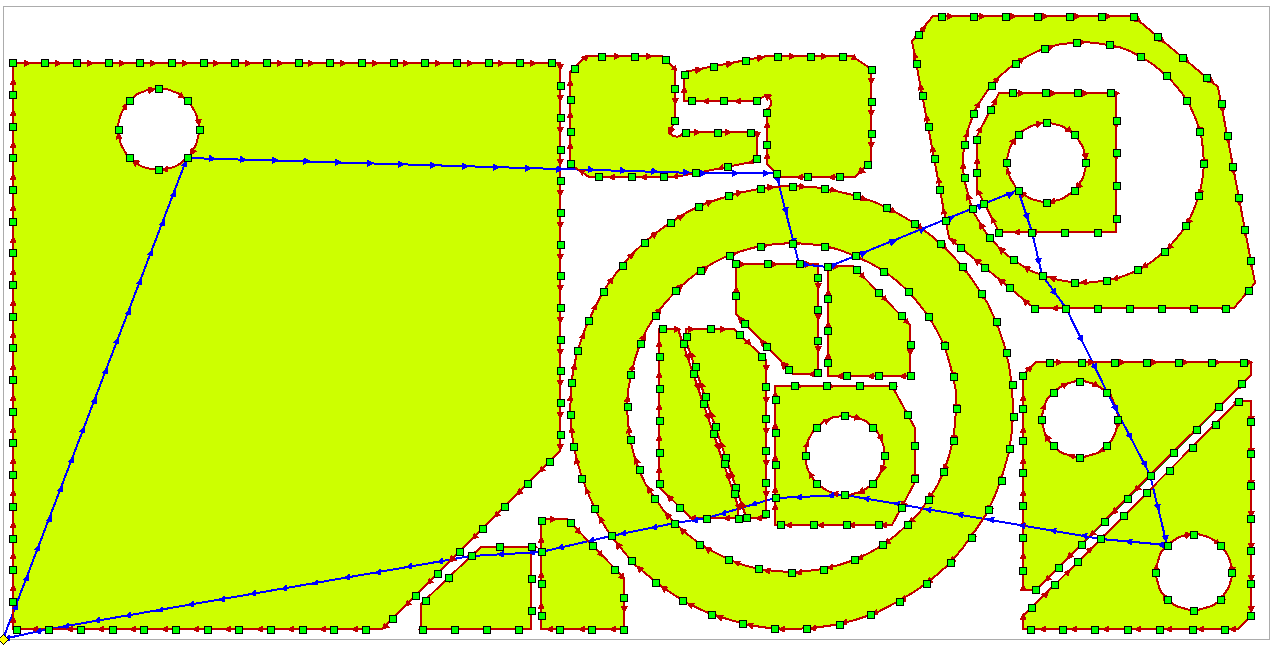
\includegraphics[width=0.95\textwidth]{464-gtsp.png}
  \end{center}
  \caption{Точное решение задачи GTSP для задания № 464}
  \label{gtsp-path}
\end{figure}

\begin{figure}
  \begin{center}
    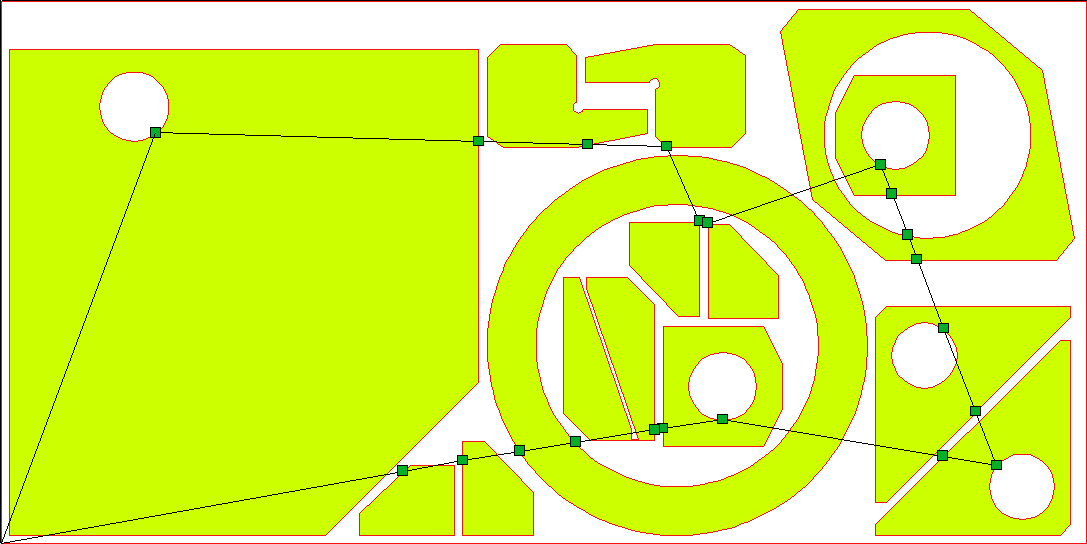
\includegraphics[width=0.95\textwidth]{464-ccp.png}
  \end{center}
  \caption{Решение задачи непрерывной резки для задания № 464}
  \label{ccp-path}
\end{figure}

\section{Заключение}

\printbibliography[heading=bibintoc]
\nocite{*}

\end{document}
